\documentclass{standalone}
\usepackage{tikz}
\usetikzlibrary{trees,fit,backgrounds,positioning}

\begin{document}

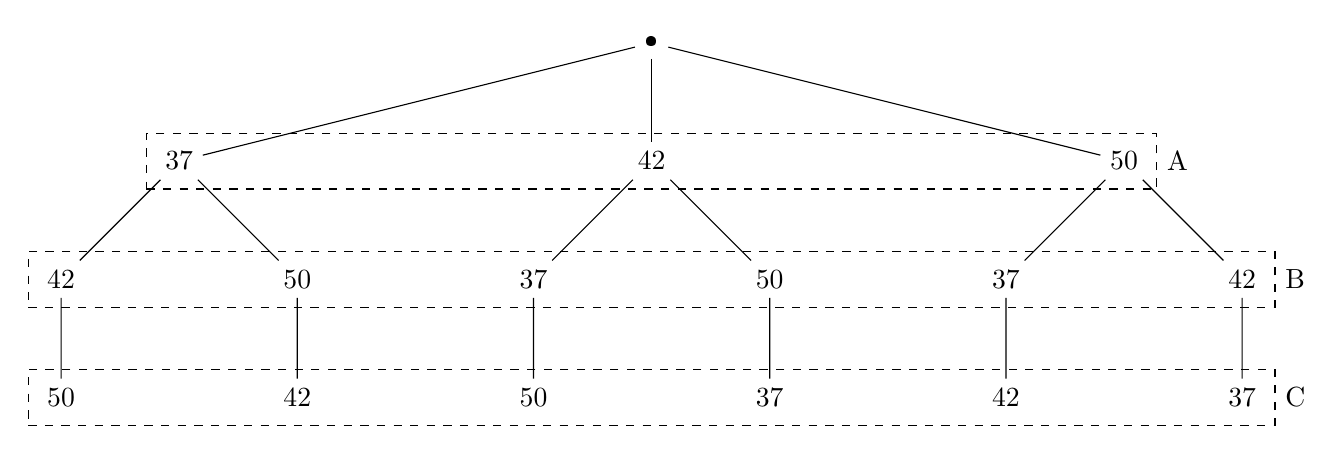
\begin{tikzpicture}[
  level distance=1.5cm,
  level 1/.style={sibling distance=6cm},
  level 2/.style={sibling distance=3cm},
  level 3/.style={sibling distance=1.5cm}
]

% Define nodes with names to reference them later for grouping
\node (root) {•}
  child {
    node (A1) {37}
      child {
        node (B1) {42}
          child {node (C1) {50}}
      }
      child {
        node (B2) {50}
          child {node (C2) {42}}
      }
  }
  child {
    node (A2) {42}
      child {
        node (B3) {37}
          child {node (C3) {50}}
      }
      child {
        node (B4) {50}
          child {node (C4) {37}}
      }
  }
  child {
    node (A3) {50}
      child {
        node (B5) {37}
          child {node (C5) {42}}
      }
      child {
        node (B6) {42}
          child {node (C6) {37}}
      }
  };

% Draw ellipses around each level with right-aligned labels
\begin{scope}[on background layer]
  \node[draw, dashed, fit=(A1)(A2)(A3), label=right:A] {};
  \node[draw, dashed, fit=(B1)(B2)(B3)(B4)(B5)(B6), label=right:B] {};
  \node[draw, dashed, fit=(C1)(C2)(C3)(C4)(C5)(C6), label=right:C] {};
\end{scope}

\end{tikzpicture}

\end{document}

